
% ----------------------------------------------------------------------
%  Set the document class
% ----------------------------------------------------------------------
\documentclass[11pt,a4paper,twoside]{article}

% ----------------------------------------------------------------------
% Define external packages, language, margins, fonts and new commands
% ----------------------------------------------------------------------
%\input{preamble} 
\usepackage[utf8]{inputenc}   % <<<<< Linux
\usepackage[english]{babel} % <<<<< English
\usepackage{notoccite}
\usepackage[skip=0.5\baselineskip]{caption}
\hyphenation{GTKWave}
\usepackage{listings}
\usepackage[all]{nowidow}
\usepackage{amsmath} %Matrix package
\usepackage{csvsimple} %csv reading package
\usepackage{authblk} %author information

\usepackage{graphicx}
\graphicspath{{./}{../../figlib/}{../mat/}{../sim/}}
\def\FontLn{% 16 pt normal
  \usefont{T1}{phv}{m}{n}\fontsize{16pt}{16pt}\selectfont}
\def\FontLb{% 16 pt bold
  \usefont{T1}{phv}{b}{n}\fontsize{16pt}{16pt}\selectfont}
\def\FontMn{% 14 pt normal
  \usefont{T1}{phv}{m}{n}\fontsize{14pt}{14pt}\selectfont}
\def\FontMb{% 14 pt bold
  \usefont{T1}{phv}{b}{n}\fontsize{14pt}{14pt}\selectfont}
\def\FontSn{% 12 pt normal
  \usefont{T1}{phv}{m}{n}\fontsize{12pt}{12pt}\selectfont}

% Use Arial font as default
%
\renewcommand{\rmdefault}{phv}
\renewcommand{\sfdefault}{phv}
\usepackage{geometry}	
\geometry{verbose,tmargin=2.5cm,bmargin=2.5cm,lmargin=2.5cm,rmargin=2.5cm}

%\usepackage{setspace}
%\renewcommand{\baselinestretch}{1.5}

\usepackage[pdftex]{hyperref} % enhance documents that are to be
                              % output as HTML and PDF
\hypersetup{colorlinks,       % color text of links and anchors,
                              % eliminates borders around links
%            linkcolor=red,    % color for normal internal links
            linkcolor=black,  % color for normal internal links
            anchorcolor=black,% color for anchor text
%            citecolor=green,  % color for bibliographical citations
            citecolor=black,  % color for bibliographical citations
%            filecolor=magenta,% color for URLs which open local files
            filecolor=black,  % color for URLs which open local files
%            menucolor=red,    % color for Acrobat menu items
            menucolor=black,  % color for Acrobat menu items
%            pagecolor=red,    % color for links to other pages
            pagecolor=black,  % color for links to other pages
%            urlcolor=cyan,    % color for linked URLs
            urlcolor=black,   % color for linked URLs
	          bookmarks=true,         % create PDF bookmarks
	          bookmarksopen=false,    % don't expand bookmarks
	          bookmarksnumbered=true, % number bookmarks
	          pdftitle={report},
            pdfauthor={Andre C. Marta},
%            pdfsubject={Thesis Title},
%            pdfkeywords={Thesis Keywords},
            pdfstartview=FitV,
            pdfdisplaydoctitle=true}

\usepackage[numbers,sort&compress]{natbib} % <<<<< References in numbered list [1],[2],...
\usepackage{subcaption} 
\usepackage{mdframed}

%%%%%%%%%%%%%%%%%%%%%%%%%%%%%%%%%%%%%%%%%%%%%%%%%%%%%%%%%%%%%%%%%%%%%%%%
%     Begin Document                                                   %
%%%%%%%%%%%%%%%%%%%%%%%%%%%%%%%%%%%%%%%%%%%%%%%%%%%%%%%%%%%%%%%%%%%%%%%%


\begin{document}

% Set plain page style (no headers, footer with centered page number)
\pagestyle{plain}

% Set roman numbering (i,ii,...) before the start of chapters
%\pagenumbering{roman}

% ----------------------------------------------------------------------
%  Cover page
% ----------------------------------------------------------------------
\begin{titlepage}
%%%%%%%%%%%%%%%%%%%%%%%%%%%%%%%%%%%%%%%%%%%%%%%%%%%%%%%%%%%%%%%%%%%%%%%%
%                                                                      %
%     File: frontvover.tex                                      %
%     Tex Master: report.tex                                           %
%                                                                      %
%     Author: Group 41                                           %
%     Last modified :  3 Mar 2021                                      %
%                                                                      %
%%%%%%%%%%%%%%%%%%%%%%%%%%%%%%%%%%%%%%%%%%%%%%%%%%%%%%%%%%%%%%%%%%%%%%%%

\thispagestyle {empty}

% IST Logo - Signature A
% parameters: bb=llx lly urx ury (bounding box), width=h_length, height=v_length, angle=angle, scale=factor, clip=true/false, draft=true/false. 
\includegraphics[bb=9.5cm 11cm 0cm 0cm,scale=0.29]{IST_A_CMYK_POS}

\begin{center}
%

\vspace{1.0cm}


% Title, author and degree
\vspace{1cm}
{\FontLb Circuit Theory and Electronics Fundamentals} \\ % <<<<< EDIT TITLE
\vspace{1cm}
{\FontSn Aerospace Engineering, Técnico, University of Lisbon} \\ % <<<<< EDIT COURSE
\vspace{1cm}
{\FontSn T1 Laboratory Report} \\
\vspace{1cm}
{\FontSn March 6, 2021} \\ % <<<<< EDIT DATE (corresponds to date of oral examination)
\vspace{1cm}
\author{Duarte Brito 96373 \and Henrique Caraça 96393 \and Nuno Ribeiro 96459}
\end{center}


\end{titlepage}

% ----------------------------------------------------------------------
% Dedication page (optional)
% ----------------------------------------------------------------------
%\input{dedication} 
%\cleardoublepage

% ----------------------------------------------------------------------
%  Acknowledgments (optional)
% ----------------------------------------------------------------------
%\input{acknowledgements}
%\cleardoublepage

% ----------------------------------------------------------------------
%  Abstract (both in English and Portuguese)
% ----------------------------------------------------------------------
%\input{resumo} 
%\cleardoublepage

%\input{abstract} 

% ----------------------------------------------------------------------
%  Table of contents, list of tables, list of figures and nomenclature
% ----------------------------------------------------------------------

% Table of contents
%
\tableofcontents

% List of tables
%\addcontentsline{toc}{section}{\listtablename}
%\listoftables
%\cleardoublepage 

% List of figures
%\addcontentsline{toc}{section}{\listfigurename}
%\listoffigures
%\cleardoublepage 

% Set arabic numbering (1,2,...) after preface
%
%\setcounter{page}{1}
%\pagenumbering{arabic}

% ----------------------------------------------------------------------
%  Body
% ----------------------------------------------------------------------

\section{Introduction}
\label{sec:introduction}

\indent

% state the learning objective 
The objective of this laboratory assignment is to make a Bandpass filter using an OP-AMP.

The equivalent circuit can be seen in Figure~\ref{fig:circuit}. 

This circuit is made up of an amplifier (an OP-AMP and resistors $R_3$ and $R_4$), a high pass filter (the left part, that is $C_1$ and $R_1$),  and a low pass filter (the right part, that is $R_2$ and $C_2$) .

In Section~\ref{sec:simulation analysis}, the circuit is analysed by
means of a ngspice simulation. In Section~\ref{sec:theoretical analysis}, a theoretical analysis of the circuit is
presented. The results are then compared in Section~\ref{sec:theoretical analysis}. The conclusions of this study are outlined in Section~\ref{sec:conclusion}.



\begin{figure}[h!] \centering
	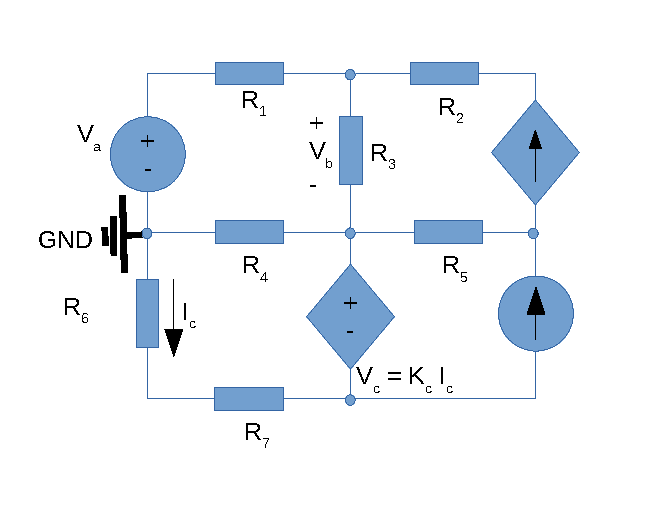
\includegraphics[width=0.6\linewidth]{circ.pdf}
	\caption{Used Circuit.}
	\label{fig:circuit}
\end{figure}







\section{Theoretical Analysis}
\label{sec:analysis}

In this section, the circuit shown in Figure~\ref{fig:circuit} is analysed
theoretically, in terms of its time and frequency responses.

\subsection{Mesh Analysis}

\begin{figure}
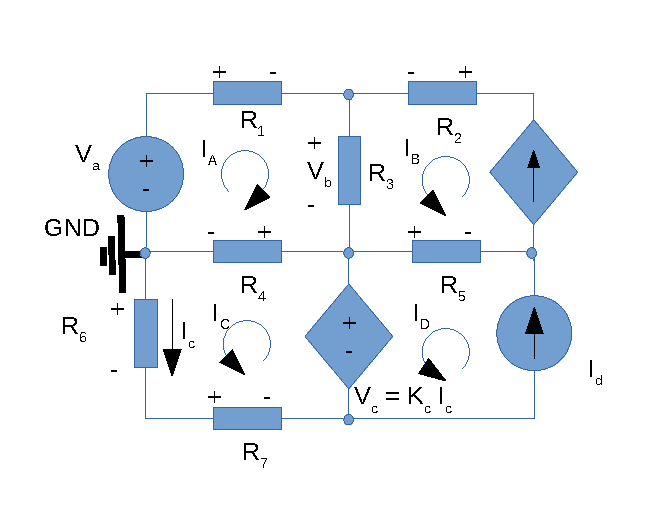
\includegraphics[width=0.4\linewidth]{circ_mesh.pdf}
\caption{Mesh Analysis}
\label{fig:circuitMesh}
\end{figure}

The Figure~\ref{fig:circuitMesh} has both the mesh's currents and the 
component's admited direction.
This reference is indispensable for the Mesh Analysis.
Using KVL in each of the 4 meshes, we achieve the following equations:

Malha A:
$$ R_1 * I_A + R_3(I_A+I_B) + R_4(I_A+I_C) = V_A$$
Malha B:
$$ I_B = K_c * R_3(I_A + I_B) $$
Malha C:
$$ R_4(I_A + I_C) + R_6 * I_C + R_7 * I_C = K_c * I_C $$
Malha D:
$$ I_D = I_d $$

After doing some algebra, we can get the following system of equations. After that, 
we can solve it by enquadrating it in a matriz like shown bellow:

\[
\begin{bmatrix}
R_1 + R_3 + R_4 & R_3 & R_4 & 0\\
K_b * R_3 & K_b * R_3 - 1 & 0 & 0\\
R_4 & 0 & R_6 - K_c + R_7 - R_4 & 0\\
0 & 0 & 0 & 1\\
\end{bmatrix}
\cdot
\begin{bmatrix}
I_A\\
I_B\\
I_C\\
I_D\\
\end{bmatrix}
=
\begin{bmatrix}
V_a\\
0\\
0\\
I_d\\
\end{bmatrix}
\]

After solving these equations using octave, we get 
the following results:

\csvautotabular{../mat/malhas.csv}

To get the current in each resistor, we use the following equations:

$$ I_1 = I_A $$
$$ I_2 = I_B $$
$$ I_3 = I_A + I_B $$
$$ I_4 = I_A + I_C $$
$$ I_5 = I_B - I_D $$
$$ I_6 = I_C $$
$$ I_7 = I_C $$

Leading to the results bellow:

\csvautotabular{../mat/cur.csv}

\subsection{Nodal Analysis}

\begin{figure}
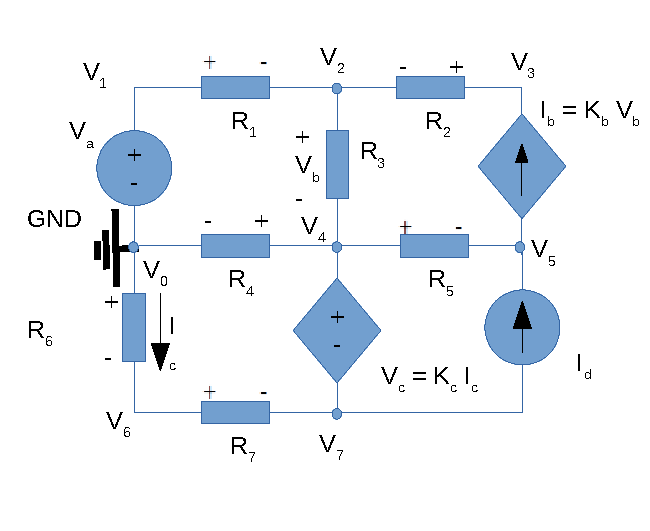
\includegraphics[width=0.4\linewidth]{circ_node.pdf}
\caption{Nodal Analysis}
\label{fig:circuitNodes}
\end{figure}

The Figure~\ref{fig:circuitNodes} has the node references appended.
This reference is indispensable for the Nodal Analysis.
Using KVL in each of the 4 meshes, we achieve the following equations:

Node 2:
$$ (V_1 - V_2)G_1 + (V_3 - V_2)G_2 = (V_2 - V_4)G_3 $$
Node 3:
$$ (V_3 - V_2)G_2 = K_b(V_2 - V_4) $$

Node 5:
$$ (V_4 - V_5)G_5 + I_d = K_b(V_2 - V_4) $$

Node 6:
$$ (V_0 - V_6)G_6 = (V_6 - V_7)G_7 $$

Additional equation:
$$ V_0 = 0 $$
$$ (V_1 - V_0) = V_a $$
$$ V_4 - V_7 = K_c(V_0 - V_6)G_6$$
$$ (V_0 -V_6)G_6 - (V_4 - V_0)G_4 + (V_1 - V_2)G_1 = 0 $$

Similarly to the last example, the algebric manipulation brings us to the following system of equations, 
and the solution can be found by enquadrating it in a matriz like shown bellow:

\[
\begin{bmatrix}
1 & 0 & 0 & 0 & 0 & 0 & 0\\
0 & 0 & 0 & 1 & 0 & K_c * G_6 & -1\\
G_1 & -G_1-G_2 - G_3 & G_2 & G_3 & 0 & 0 & 0\\
0 & -K_b & 0 & G_5 + K_b & -G_5 & 0 & 0\\
0 & -K_b & 0 & G_5 + K_b & -G_5 & 0 & 0\\
0 & 0 & 0 & 0 & 0 & -G_6-G_7 & G_7\\
G_1 & -G_1 & 0 & -G_4 & 0 & -G_6 & 0\\
\end{bmatrix}
\cdot
\begin{bmatrix}
V_1\\
V_2\\
V_3\\
V_4\\
V_5\\
V_6\\
V_7\\
\end{bmatrix}
=
\begin{bmatrix}
V_a\\
0\\
0\\
0\\
-I_d\\
0\\
0\\
\end{bmatrix}
\]

After solving these equations using octave, we get 
the following results:

\csvautotabular{../mat/nos.csv}

\subsection{Result Comparison }

\section{Simulation Analysis}
\label{sec:simulation}

\subsection{Operating Point Analysis}

Table~\ref{tab:op} shows the simulated operating point results for the circuit
under analysis. Compared to the theoretical analysis results, one notices the
following differences: describe and explain the differences.

\begin{table}[h]
  \centering
  \begin{tabular}{|l|r|}
    \hline    
    {\bf Name} & {\bf Value [A or V]} \\ \hline
    @gb[i] & -2.47520e-04\\ \hline
@id[current] & 1.005321e-03\\ \hline
@r1[i] & 2.364560e-04\\ \hline
@r2[i] & -2.47520e-04\\ \hline
@r3[i] & -1.10640e-05\\ \hline
@r4[i] & 1.201119e-03\\ \hline
@r5[i] & -1.25284e-03\\ \hline
@r6[i] & 9.646630e-04\\ \hline
@r7[i] & 9.646630e-04\\ \hline
v(1) & 5.076387e+00\\ \hline
v(2) & 4.828240e+00\\ \hline
v(3) & 4.317615e+00\\ \hline
v(4) & 4.862301e+00\\ \hline
v(5) & 8.665725e+00\\ \hline
v(6) & -1.94693e+00\\ \hline
v(7) & -2.95363e+00\\ \hline
v(9) & -1.94693e+00\\ \hline

  \end{tabular}
  \caption{Operating point. A variable preceded by @ is of type {\em current}
    and expressed in Ampere; other variables are of type {\it voltage} and expressed in
    Volt.}
  \label{tab:op}
\end{table}

\lipsum[1-1]


\subsection{Transient Analysis}

Figure~\ref{fig:trans} shows the simulated transient analysis results for the
circuit under analysis. Compared to the theoretical analysis results, one
notices the following differences: describe and explain the differences.

\begin{figure}[h] \centering
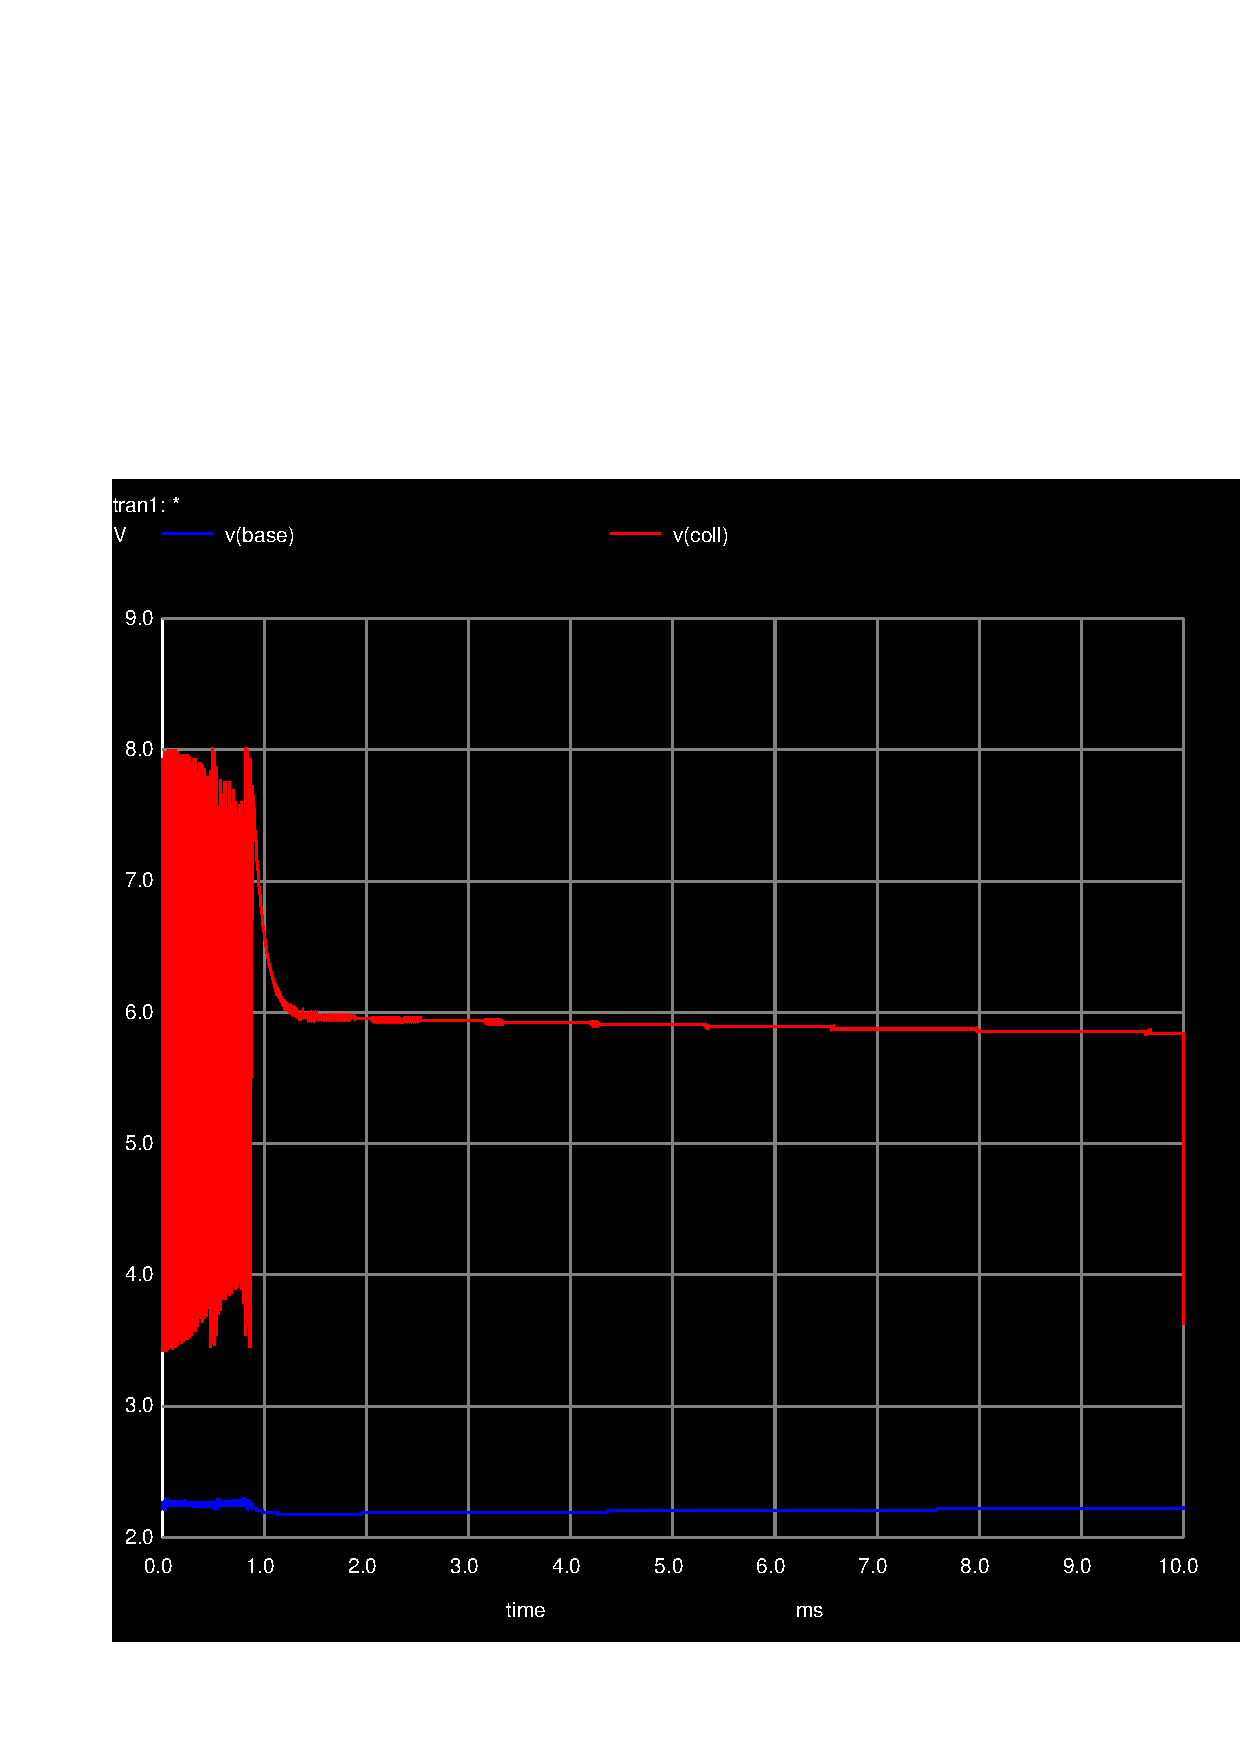
\includegraphics[width=0.6\linewidth]{trans.pdf}
\caption{Transient output voltage}
\label{fig:trans}
\end{figure}

\lipsum[1-1]



\subsection{Frequency Analysis}

\subsubsection{Magnitude Response}

Figure~\ref{fig:acm} shows the magnitude of the frequency response for the
circuit under analysis. Compared to the theoretical analysis results, one
notices the following differences: describe and explain the differences.

\begin{figure}[h] \centering
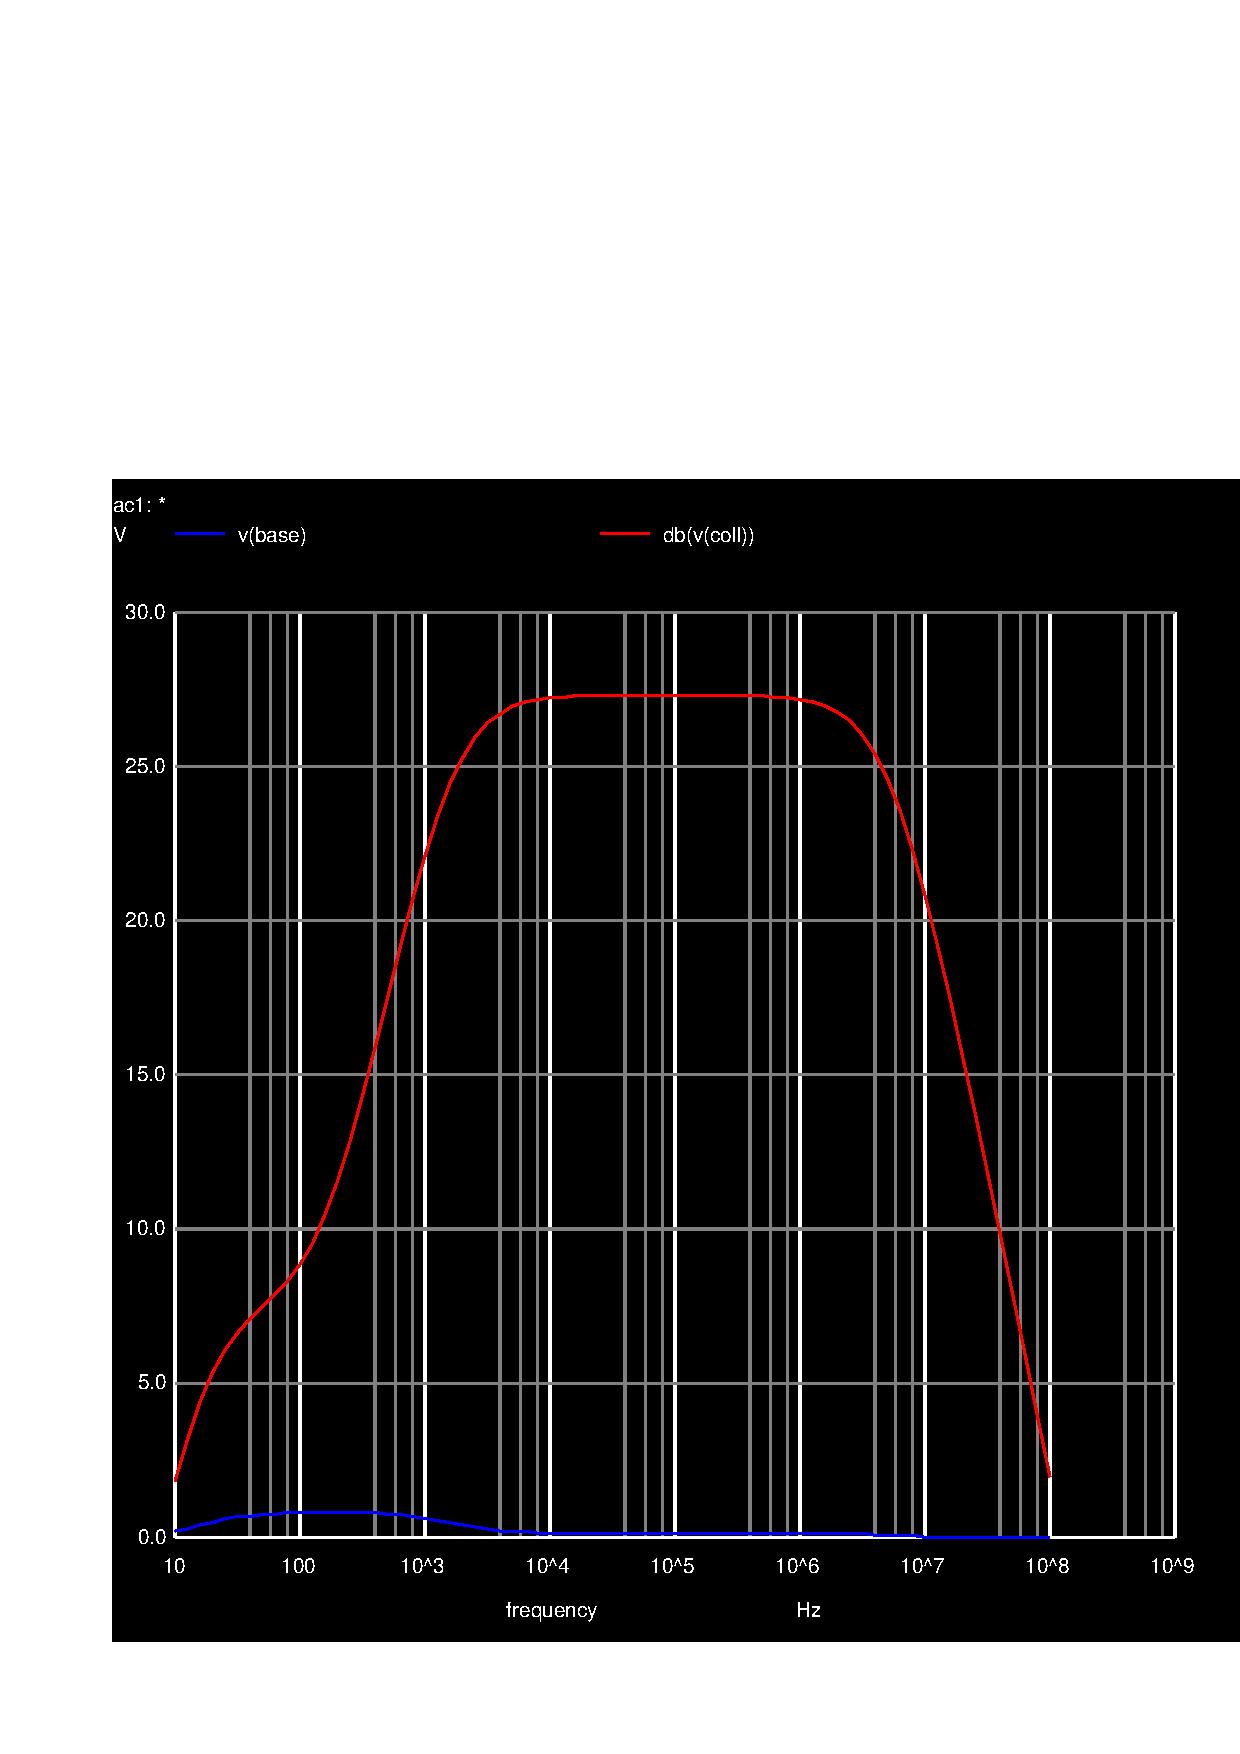
\includegraphics[width=0.6\linewidth]{acm.pdf}
\caption{Magnitude response}
\label{fig:acm}
\end{figure}

\lipsum[1-1]

\subsubsection{Phase Response}

Figure~\ref{fig:acp} shows the magnitude of the frequency response for the
circuit under analysis. Compared to the theoretical analysis results, one
notices the following differences: describe and explain the differences.

\begin{figure}[h] \centering
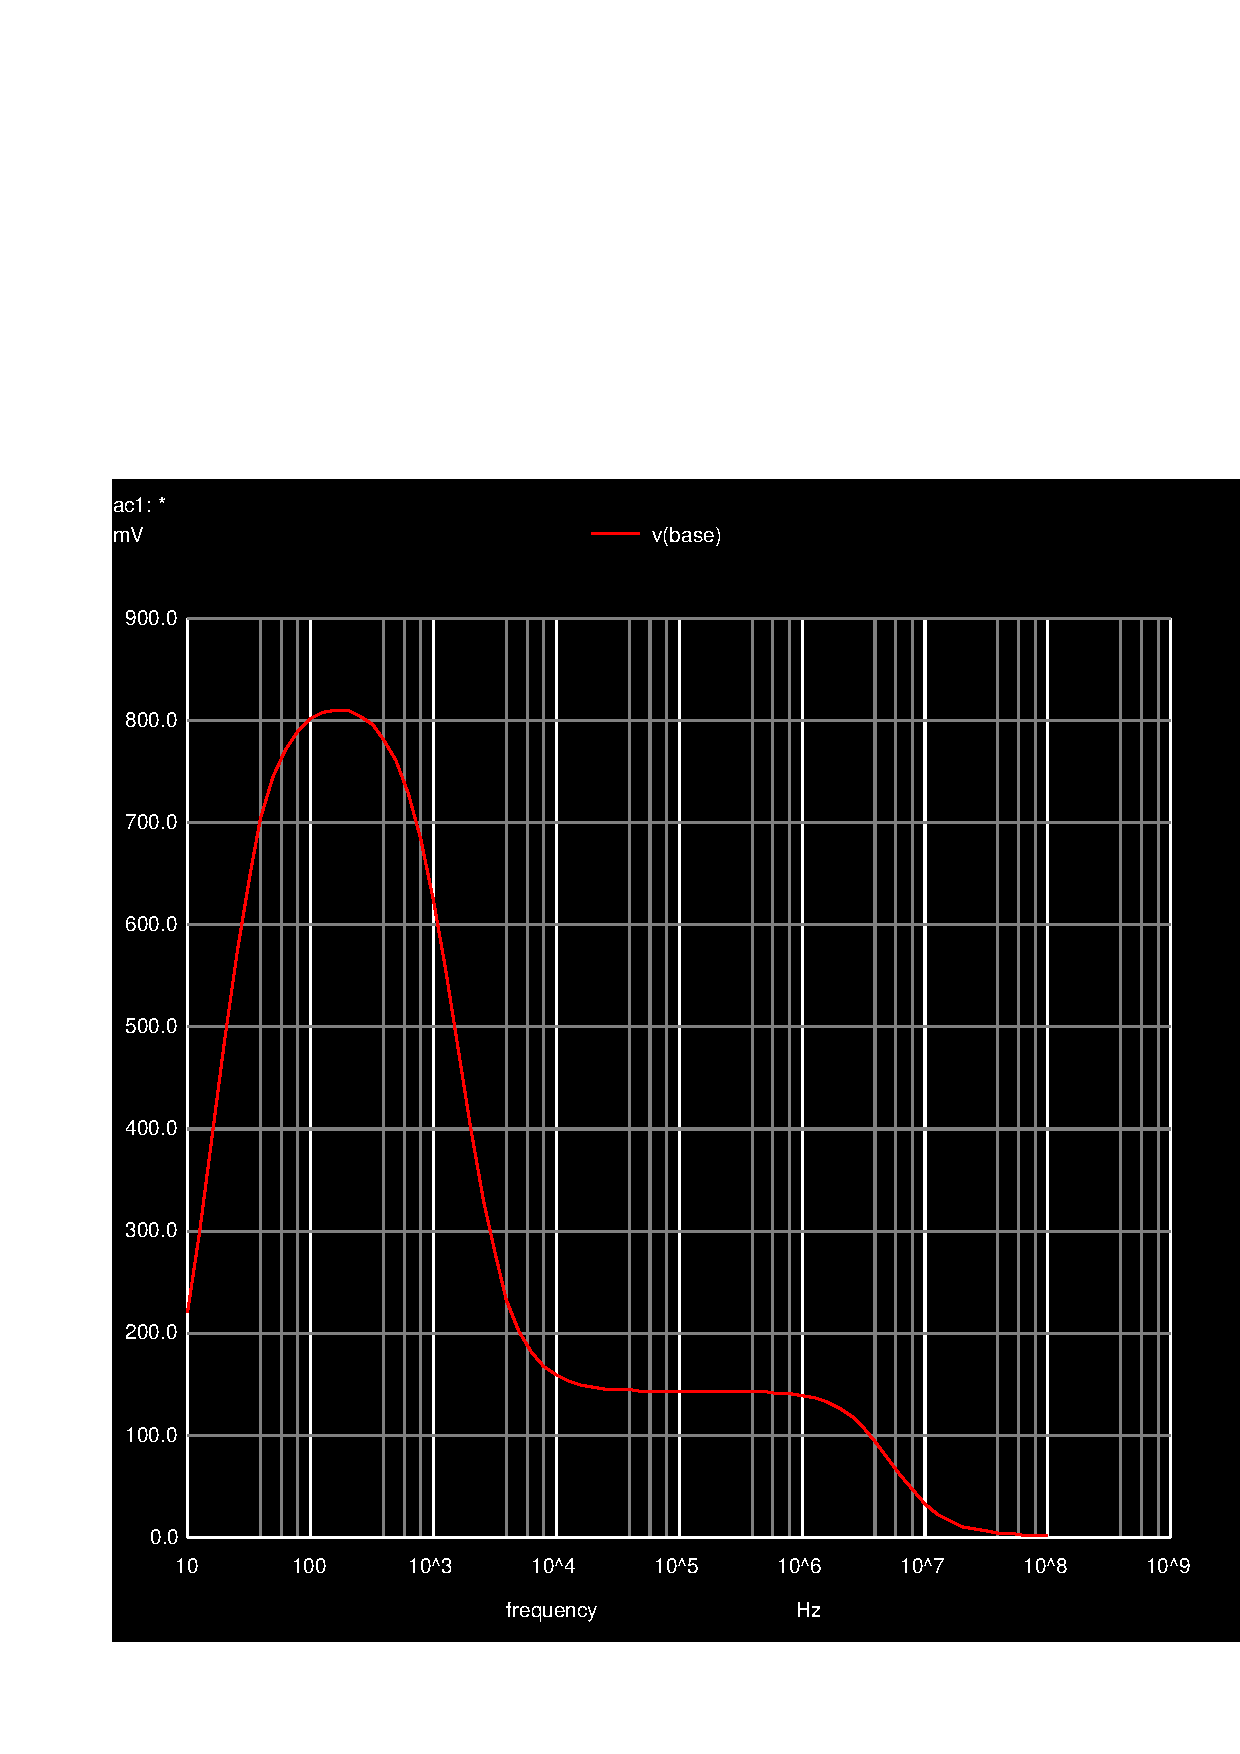
\includegraphics[width=0.6\linewidth]{acp.pdf}
\caption{Phase response}
\label{fig:acp}
\end{figure}

\lipsum[1-1]

\subsubsection{Input Impedance}

Figure~\ref{fig:zim} shows the magnitude of the frequency response for the
circuit under analysis. Compared to the theoretical analysis results, one
notices the following differences: describe and explain the differences.

\begin{figure}[h] \centering
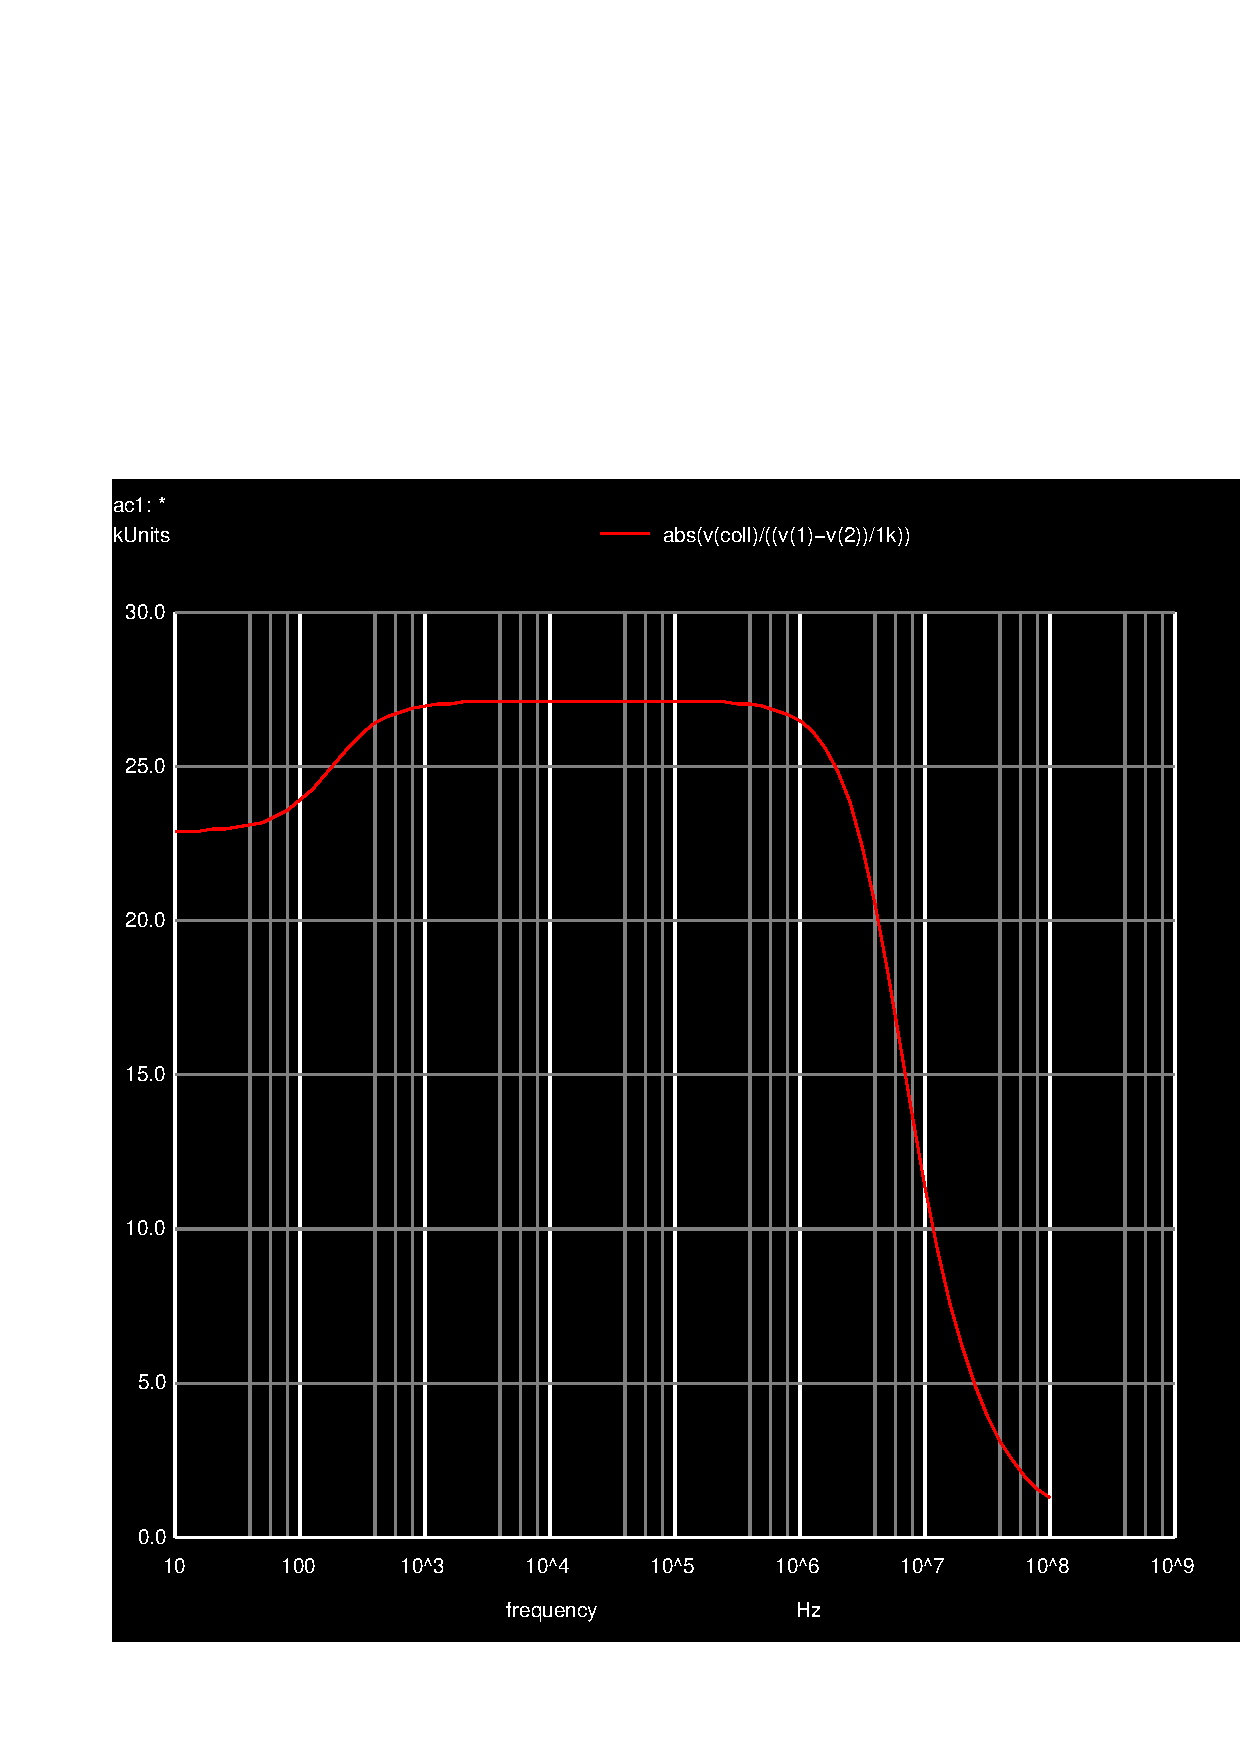
\includegraphics[width=0.6\linewidth]{zim.pdf}
\caption{Input impedance}
\label{fig:zim}
\end{figure}

\lipsum[1-1]





\section{Conclusion}
\label{sec:conclusion}


\par Unlike previous laboratories, this time, the results were not equal.

However, we believe that the differences are not that significant and they can be explained by how NGSpice solves the circuit compared to how it was done in the theoretical analysis.

To solve the circuit, NGSpice used far more advanced simulation methods for the diodes, with many more parameters, while we used an approximated model with $V_{on}$ and an incremental resistor. 

This way, the objective should have never been to have equal results, but rather, have results that are "close enough", which we believe it was achieved.


%To sum up, we believe that the goals of this report were achieved.

%\cleardoublepage

% ----------------------------------------------------------------------
%  Bibliography
% ----------------------------------------------------------------------
%\addcontentsline{toc}{section}{\bibname}
%\bibliographystyle{abbrvunsrtnat} % <<<<< SELECT IF USING REFERENCES BY NUMBER (CITATION ORDER)
%\bibliography{../../../BIBfile.bib}

% ----------------------------------------------------------------------
\end{document}
% ----------------------------------------------------------------------
